\pagebreak
\clearpage
\section{Supplementary Material}
\label{sec:sm}

\begin{figure}
\centering
\subfloat[]{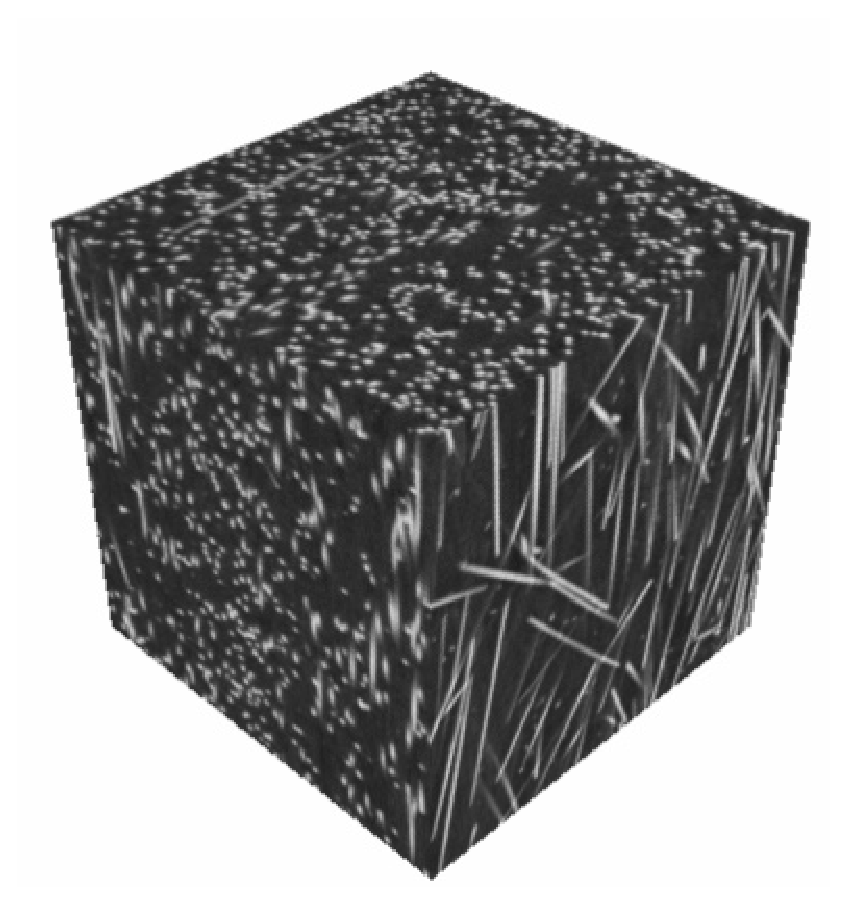
\includegraphics[width=0.25\linewidth]{imagesMT2014/glass-scalar.eps}}
  \subfloat[]{\includegraphics[width=0.25\linewidth]{imagesMT2014/glass-scalar-slice}}
  \subfloat[]{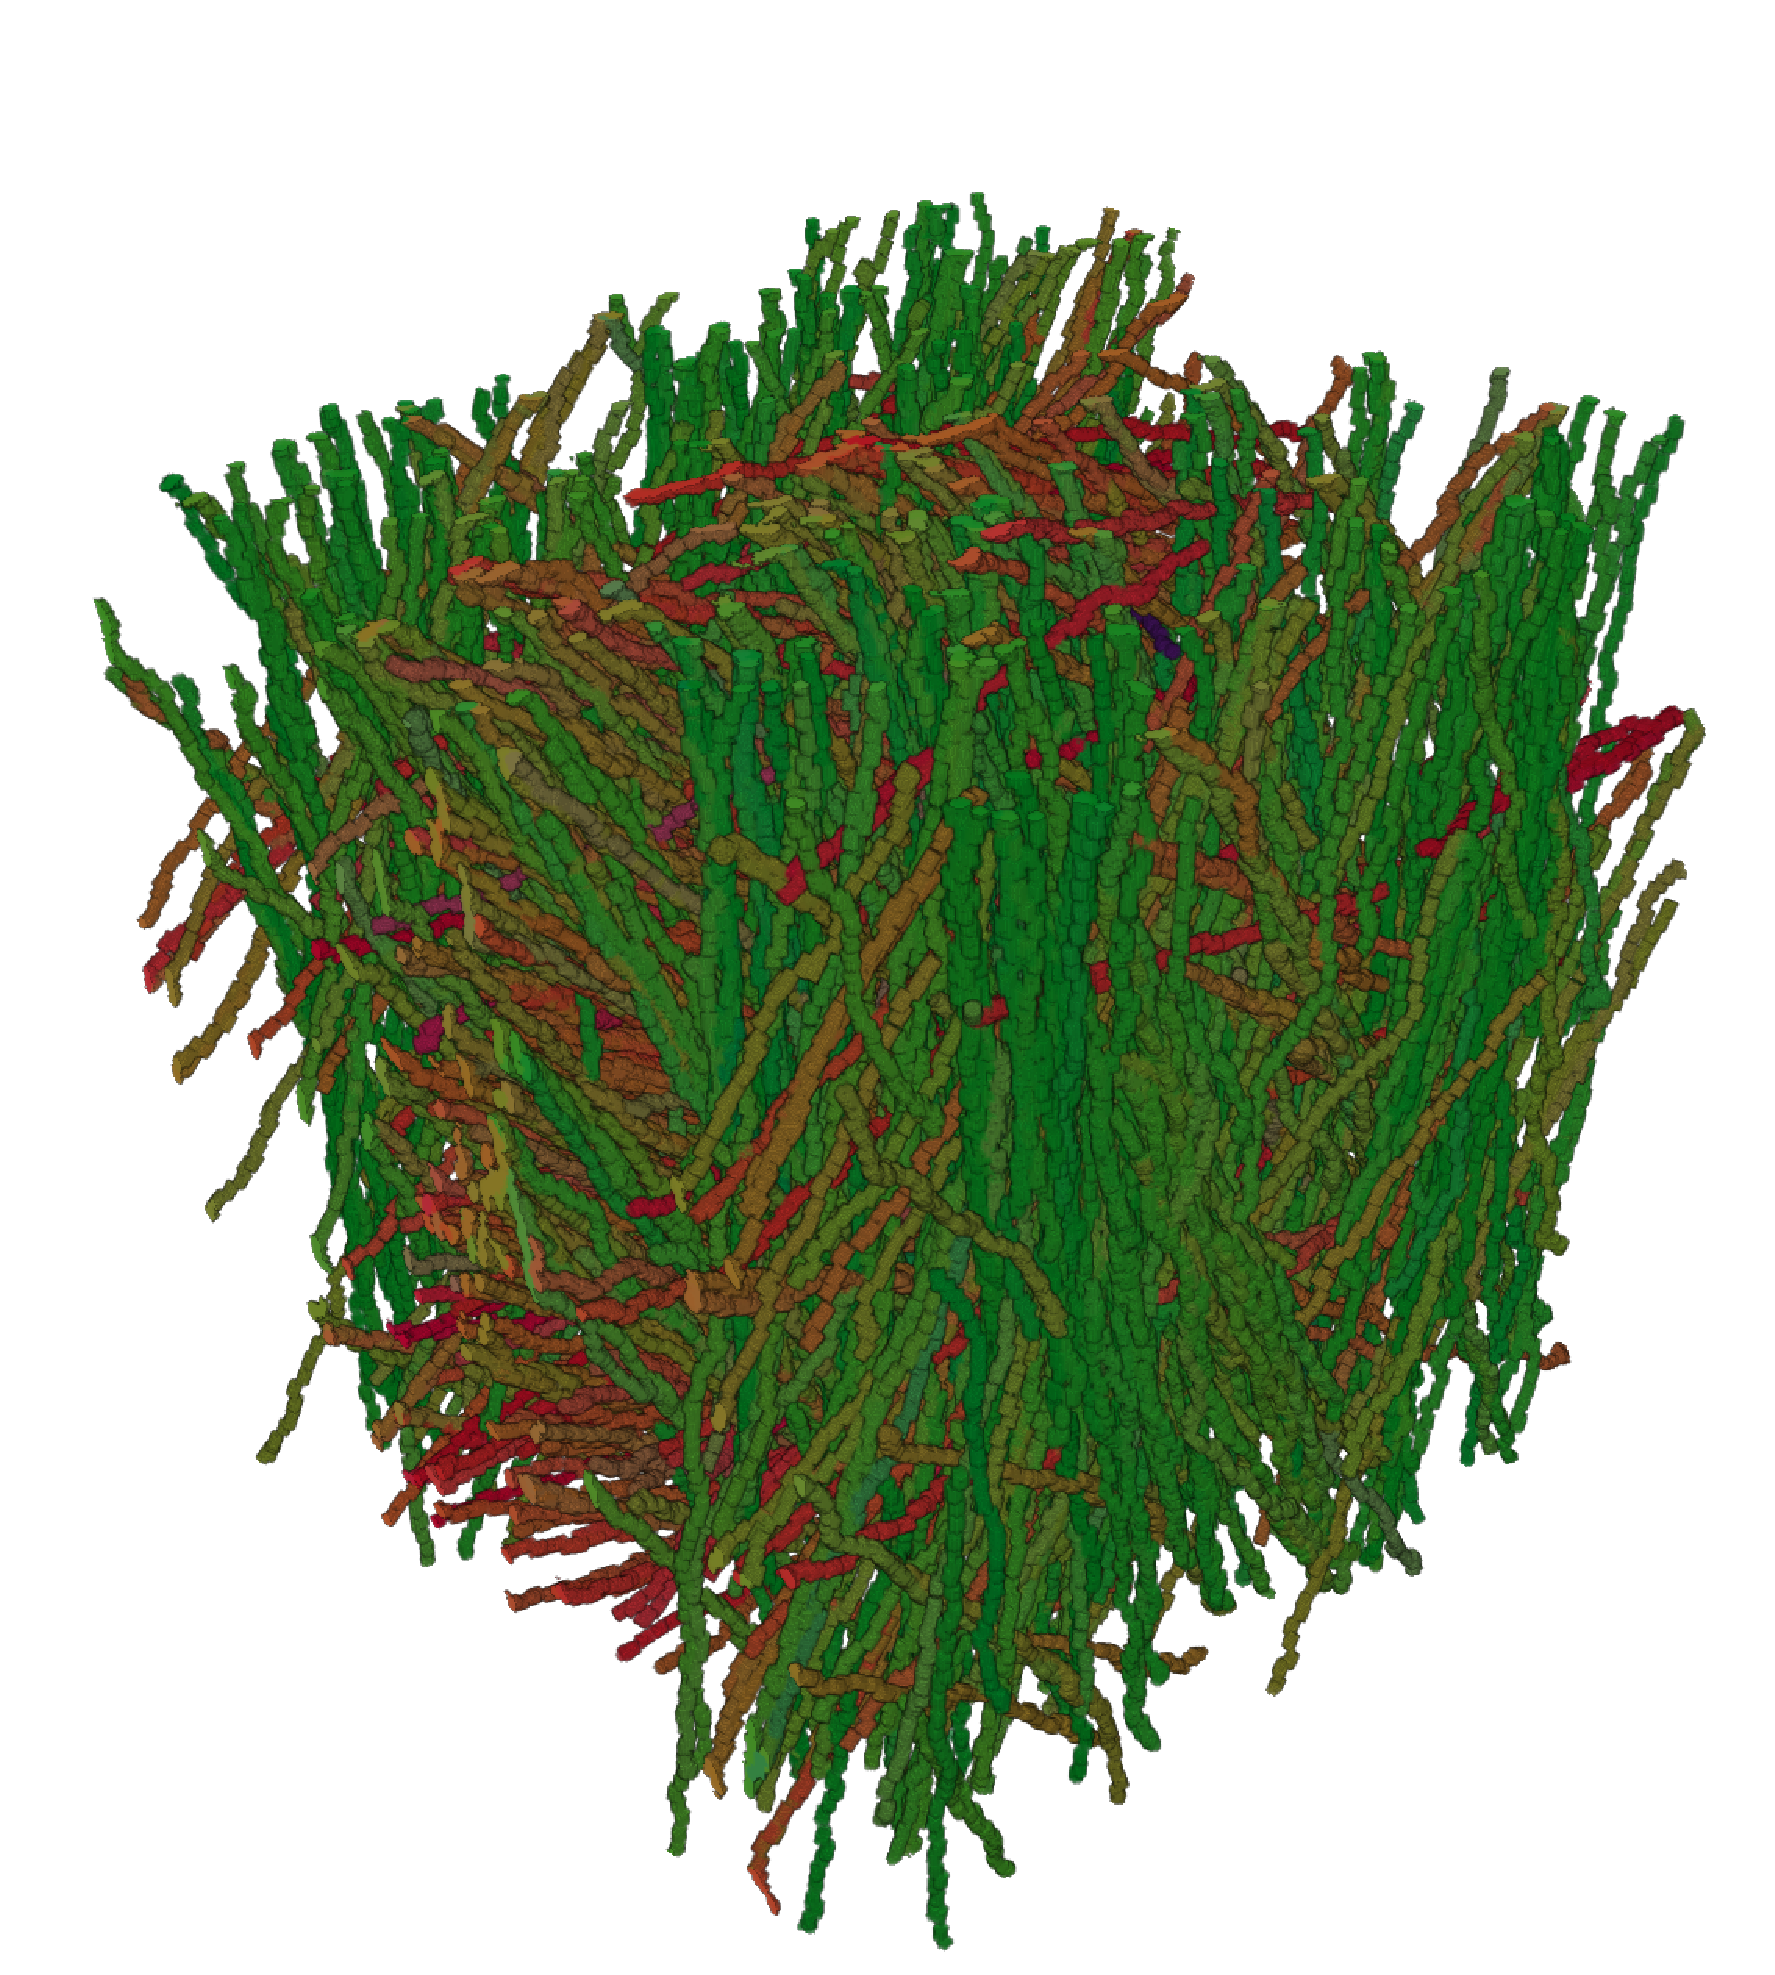
\includegraphics[width=0.25\linewidth]{imagesMT2014/glass-cluster-b.eps}}
  \subfloat[]{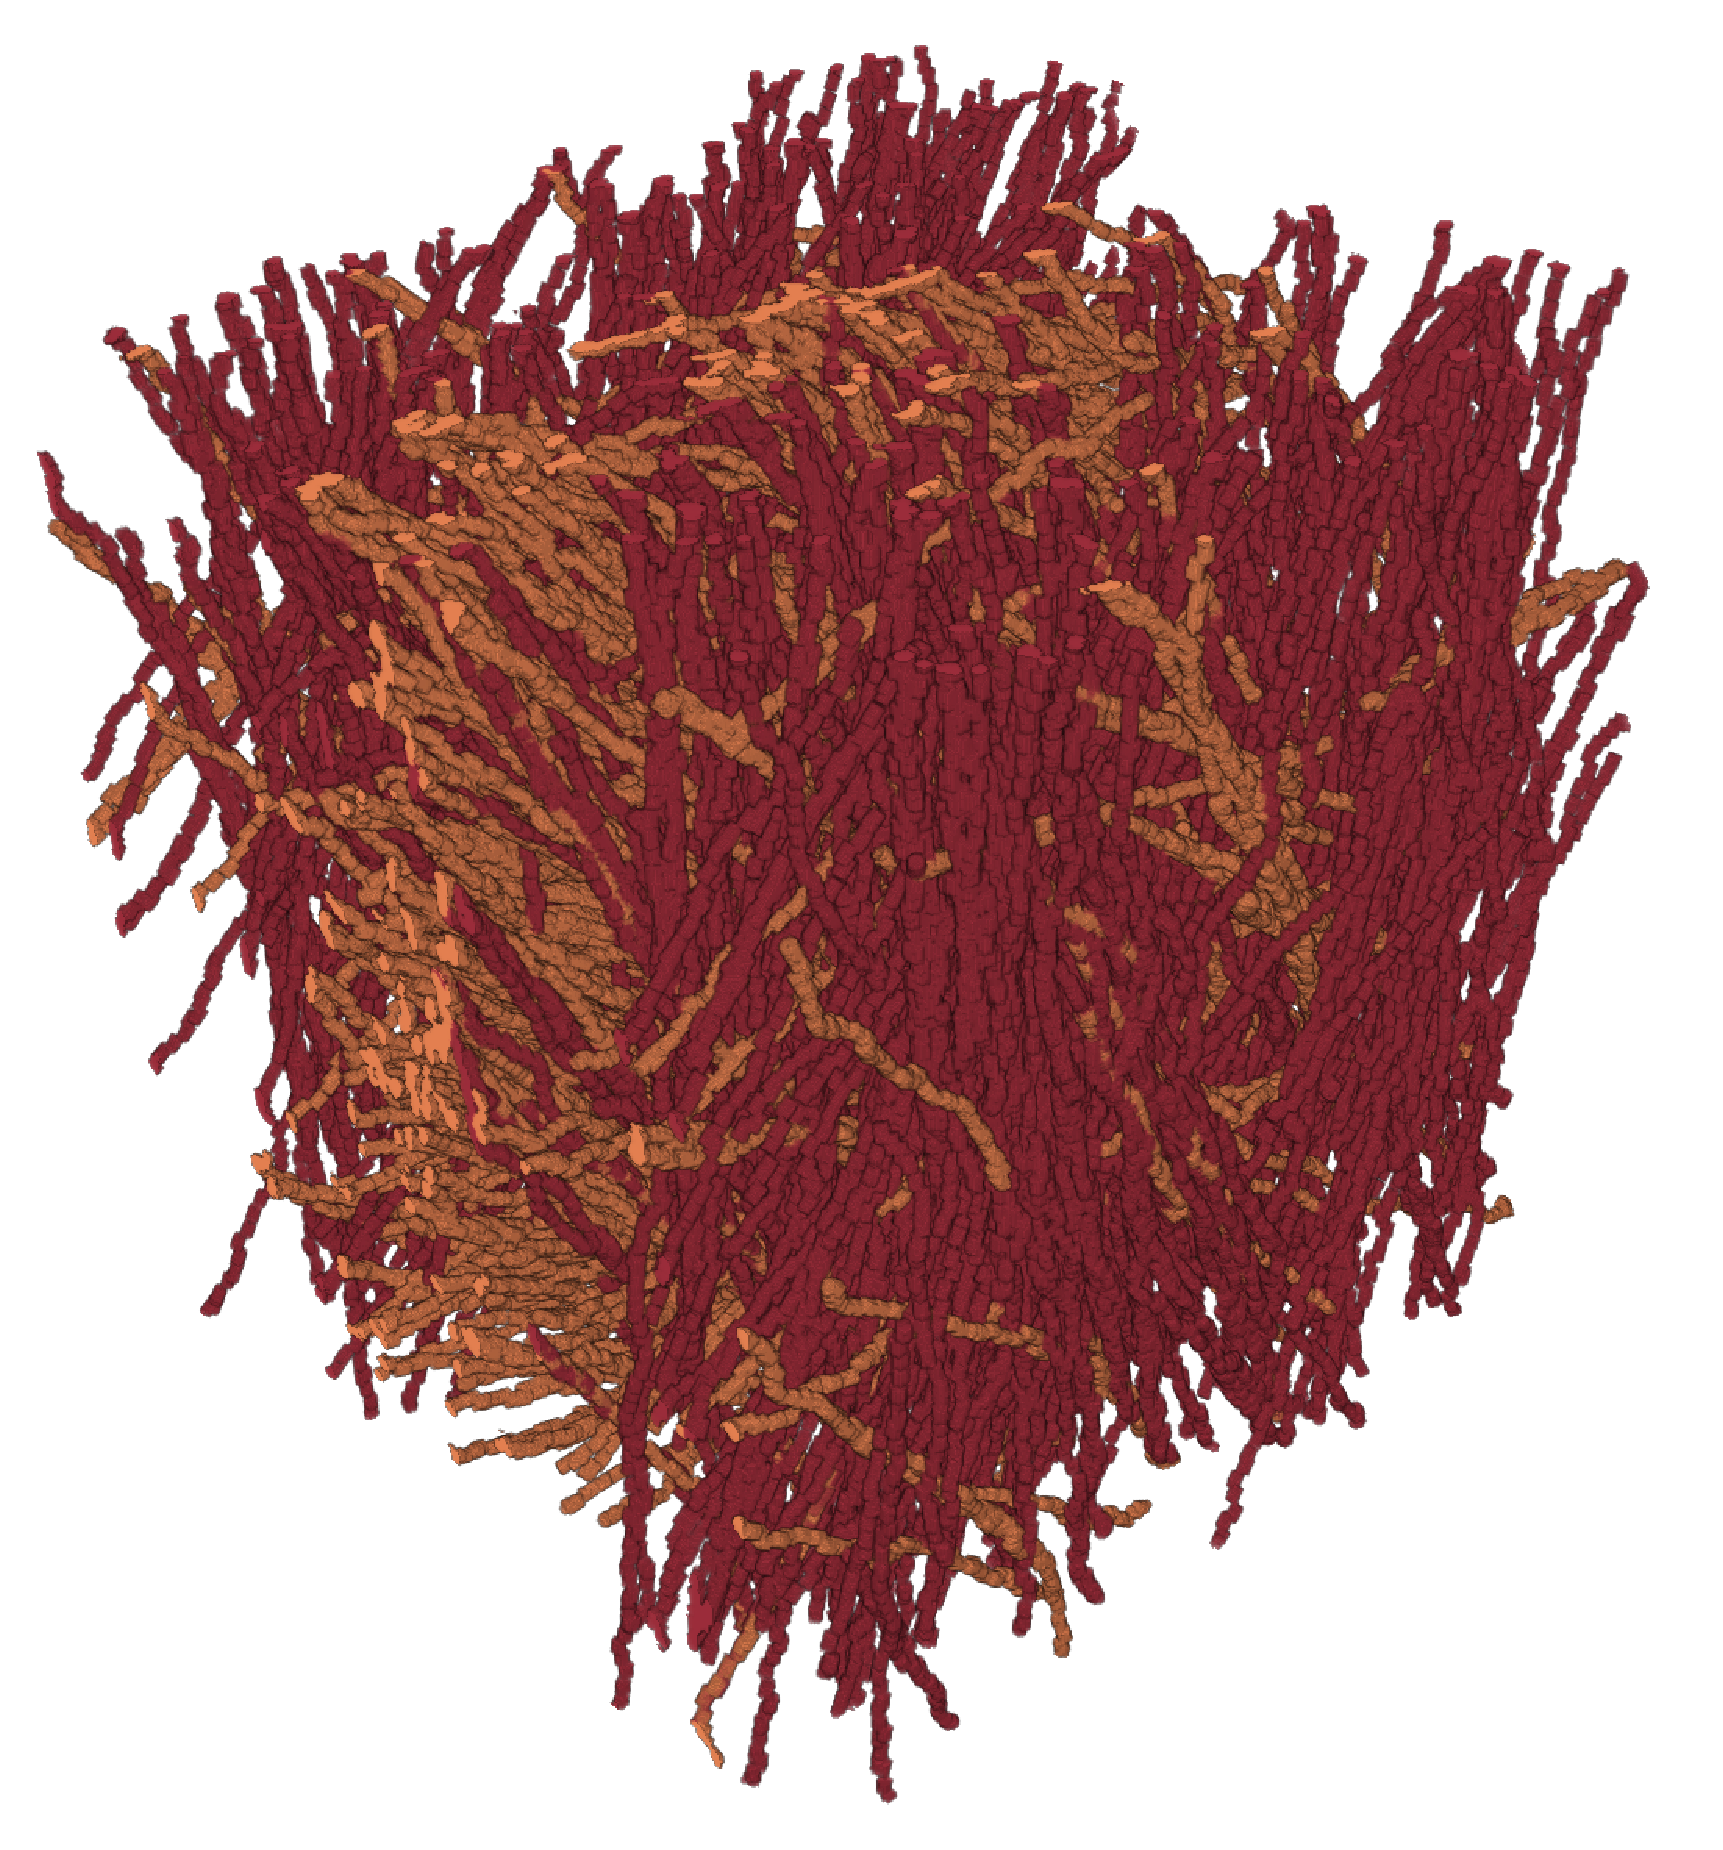
\includegraphics[width=0.25\linewidth]{imagesMT2014/glass-cluster-a.eps}}
  \caption{Our algorithm on a data set made of glass fibers. (a) The scalar dataset, (b) Depicts a slice from the data set, the  fibers are clearly demarcated from the rest of the matrix as oppose to the type of data  where it is hard to distinguish the fibers (Fig.~\ref{fig:data-char} or Fig.~\ref{fig:prepreg}A). (c) The result of the MetaTracts process, the colors are to help visualization. (d) The result of the orientation based clustering, the two clusters are marked red and yellow.}\label{fig:glass}
\end{figure}
\subsection{Glass Fibers}
One simple way we used to validate the accuracy of shape and size of the extracted MetaTracts, is to run the MetaTract technique on Glass fibers.
Unlike the presented data, in glass the fibers are clearly visible (Fig.~\ref{fig:glass}(a)). We noted that the extracted MetaTracts closely followed the fibers in the data.
\subsection{Voxelization and surface extraction Extended}
The voxelization results and some of the meshes extracted from our second data set (Fig.~\ref{fig:prepreg}) are shown in Fig.~\ref{fig:vox_extended}.
\begin{figure}[h]
\centering

\subfloat[]{\includegraphics[width=0.2\textwidth]{imagesMT2014/crop-6-C2-vol}}
\subfloat[]{\includegraphics[width=0.2\textwidth]{imagesMT2014/mesh_prepreg_A}}
\\
\caption{(a) Voxelization of Fig.~\ref{fig:prepreg}C, (b) Shows some of the extracted meshes.}
\label{fig:vox_extended}
\end{figure}
\subsection{Robustness to parameter changes}
Figure~\ref{fig:radius_3} shows the results of data set in Fig.~\ref{fig:data-char} clustered into 2 orientation cluster, and each orientation further clustered into 15 clusters (instead of 10 in Fig.~\ref{fig:len_dist_crop16}). Fig.~\ref{fig:radius_3}(a) shows the number of tracts, the median, minimum and maximum length of the MetaTracts in orientation cluster Fig.~\ref{fig:orientation_clustering}C.
The ground truth is 5 bundles. The radius of the individual MetaTract has been set to 3. We see that similar to Fig~\ref{fig:len_dist_crop16} the correct bundles are identified even with overestimated `h'. The median lengths of the extracted bundles are also similar. Fig~\ref{fig:radius_3}(c, d) shows the individual orientation bundles and Fig~\ref{fig:radius_3}(b) shows the combined bundles.
\begin{figure}[h]
\centering
\subfloat[]{\includegraphics[width=0.6\textwidth]{imagesMT2014/Graph_crop16_3}}\\
\subfloat[]{\includegraphics[width=0.3\textwidth]{imagesMT2014/crop-16/radius_3_orientC}}\\
\subfloat[]{\includegraphics[width=0.25\textwidth]{imagesMT2014/crop-16/radius_3_orientA}}
\subfloat[]{\includegraphics[width=0.25\textwidth]{imagesMT2014/crop-16/radius_3_orientB}}
\caption{(a) Number of tracts and median, minimum and maximum length of individual MetaTracts in the orientation cluster Fig.~\ref{fig:orientation_clustering}C, clustered into 15 clusters (Fig.~\ref{fig:crop-16-decomp}A top). The unit for length is the grid cube length.(b) shows the combined clusters from both the orientation, (c),(d) show the clustering of each orientation.}
\label{fig:radius_3}
\end{figure}